\documentclass{article}
\usepackage{hyperref}
\usepackage[most]{tcolorbox}
\usepackage[T1]{fontenc}
\usepackage{lmodern} 
\usepackage{lipsum}
\usepackage{graphicx}

\renewcommand{\contentsname}{Tabla de Contenidos}


\graphicspath{ {./images/} }


\title{Simulando una sociedad a partir del dilema del prisionero}
\author{Carlos Mario Chang Jardinez C312\\Ernesto Rousell Zurita C312\\Carlos Manuel Garc\'{\i}a Rodr\'{\i}guez C312\\\\	
\small{\sc Ciencia de la Computaci\'on}\\
\small{\sc Facultad de Matem\'atica y Computaci\'on}\\
\small{\sc Universidad de La Habana. Cuba}
}

\begin{document}

\maketitle
\newpage
\tableofcontents
\newpage

\section{Introduci\'on}
La l\'{\i}nea de este trabajo comenz\'o con la siguiente idea: ¿Que pasar\'{\i}a si pudieramos simular diferentes civilizaciones, por
decirlo de alguna manera, con diferentes ideolog\'{\i}as, tipo de gobierno, recursos, entorno. Y a la vez cada civilizaci\'on tendria
personas con diferentes formas de pensar, actuar y relacionarse, con moralidades diferentes?. ¿Y si pudieramos comparar pseudo-objetivamente
a esas civilizaciones en base a la cantidad de d\'{\i}as que sobreviven?. No fue dif\'{\i}cil darse cuenta que era una idea muy ambiciosa, y por
tanto irrealizable como tema de este trabajo. Sin embargo, esa idea sirvi\'o de inspiraci\'on para lo que finalmente se realiz\'o.

\subsection*{¿En qu\'e consiste el dilema del prisionero?}
El dilema del prisionero es un problema muy conocido en la teor\'{\i}a de juegos. Se plantea de la siguiente manera: dos personas son arrestadas por
un crimen que cometieron juntas. Cada una es interrogada por separado y se les propone que traicionen y delaten al otro a cambio de una reducci\'on de
la condena, entonces las diferentes opciones que tienen ante s\'{\i} los criminales son las siguientes:

\begin{itemize}
      \item Si ninguno de ellos traiciona al otro ambos reciben una condena de 1 a\~no.
      \item Si uno de ellos delata al otro, el primero queda libre mientras que el otro recibe una condena de 3 a\~nos.
      \item Si ambos se delatan mutuamente reciben una condena de 2 a\~nos.
\end{itemize}
¿Entonces? ¿Qu\'e es lo m\'as conveniente para cada uno de los prisioneros?¿Y si se juegan varias veces seguidas?. Ese es el sentido del juego, este
problema es muy interesante, y existen muchos enfoques desde donde se puede ver y analizar.

Este es solo un ejemplo de una familia de juegos llamados juegos de suma no nula o juegos de suma no cero. Pero en general los otros juegos de la misma familia
tienen la misma estructura: hay dos jugadores, cada uno se enfrenta a la decisi\'on de cooperar o traicionar al otro, y cada acci\'on produce una ganancia o
p\'erdida de recursos para cada jugador. Por supuesto, en estos juegos, la estrategia \'optima es traicionar al otro jugador, ya que es la jugada que garantiza
la mayor ganancia m\'{\i}nima. Sin embargo, lo interesante de esto, es que cambia radicalmente si se juegan m\'as rondas.

\subsection*{M\'as de dos prisioneros}
Como se mencion\'o anteriormente, este trabajo se inspir\'o en la idea de simular civilizaciones. Por lo tanto, surgi\'o la idea de simplificar esto
a un dilema del prisionero con m\'as de dos jugadores, simulando as\'{\i}, de alguna manera, una civilizaci\'on. Las reglas se abordar\'an en detalle
m\'as adelante.
\newpage

\section{Reglas del juego}
\vspace*{5mm}
\subsection{Objetivo}
Cada jugador empieza con una cantidad inicial de recursos aleatorios(como en la vida real). Y cada d\'{\i}a pierde una cantidad fija de recursos, que pueden
representar perfectamente los recursos que gastaron ese d\'{\i}a con tal de sobrevivir. Cada jugador tendr\'a oportunidades de ganar o perder recursos al igual
que en el dilema del prisionero, la diferencia es que aqu\'{\i} cada ronda o juego se hace colaborativamente entre todos los jugadores de la civilizaci\'on.
El objetivo de cada juegador es simplemente sobrevivir el mayor n\'umero de d\'{\i}as posibles.

\subsection{Ronda}
Cada ronda del juego representa un d\'{\i}a de la civilizaci\'on, cada d\'{\i}a surge un evento nuevo que puede ser de diferentes tipos, cada evento intenta
simular de la forma m\'as parecida posible situaciones que podr\'{\i}an ser reales en una civilizaci\'on de este estilo.

\subsubsection{Eventos cooperativos:}
Estos eventos tienen asociado una cantidad positiva o negativa de recursos, ya que pueden ser eventos positivos o negativos. Estos tipos de eventos hacen alusi\'on a situaciones del estilo:
\begin{itemize}
      \item Ha aparecido una mina de carb\'on a 5km de distancia es necesario ir a minar el carb\'on.
      \item El trigo ha madurado y es necesario cosecharlo.
      \item Se necesita madera en la civilizaci\'on y se necesita ir a talar \'arboles.
      \item Es necesario crear pozos para tener un f\'acil acceso al agua potable en vez de acarrear agua desde el r\'{\i}o.
      \item Con el fin de conseguir carne se est\'an agrupando en el pueblo para ir de cacer\'{\i}a.
      \item Las fuertes lluvias han tra\'{\i}do inundaciones al pueblo, es necesario la colaboraci\'on de todos para reparar los destrozos.
\end{itemize}
Aqu\'{\i} los pobladores se dividen en grupos aleatoriamente, y empieza el juego. Cada uno debe tomar una decisi\'on, que puede ser: \textbf{cooperar},
\textbf{explotar} o \textbf{trabajar en solitario}. Luego esa decisi\'on se "enfrenta" con las decisiones de los otros integrantes de su grupo siguiendo la
siguiente matriz de decisisones y ganancias.
\vspace*{2mm}
\begin{center}
      \begin{tabular}{|l|c|c|c|}
            \hline
                     & Cooperar & Explotar & Solo  \\
            \hline
            Cooperar & (10,10)  & (0,15)   & (8,8) \\
            \hline
            Explotar & (15,0)   & (0,0)    & (3,8) \\
            \hline
            Solo     & (8,8)    & (8,3)    & (8,8) \\
            \hline
      \end{tabular}
\end{center}
Podemos pensarlo de la siguiente manera: Aparece una mina de carb\'on y van varios pobladores a minar. Una persona por si sola solo
puede extraer 8 puntos de recursos, si coopera con otra persona entre los dos pueden ser m\'as eficientes al especializarce y logran
extraer 20 puntos, que se reparten equitativamente. Si uno explota y el otro coopera, como hay uno que le interesa mas robar que trabajar,
entre los dos solo logran conseguir 15 puntos, pero estos solo se los queda el que decidi\'o explotar. Si ambos explotan, trabaja y no
se ponen de acuerdo as\'{\i} que nadie obtiene nada. Y si uno explota y el otro decide ir por su cuenta el que trabaja solo ya vimos que
solo puede obtener 8 puntos, y el que explota frustrado porque no puede robar pues trabaja poco y solo obtiene 3 puntos.

Y as\'{\i} cada jugador acumula puntos en base a la decisi\'on que tom\'o y las decisiones que tomaron cada uno de los otros jugadores.
Luego de eso los recursos que ten\'{\i}a asignado ese evento se reparten en base a la cantidad de puntos de cada jugador en su grupo.
Se hace evidente que el objetivo es obtener la mayor cantidad de puntos en los eventos positivos y perder la menor cantidad en los eventos
negativos.

\subsubsection{Eventos especiales: } estos son mas f\'aciles de comprender, son eventos que pueden afectar a uno o varios pobladores, rest\'andoles
o otorg\'andoles recursos de fñorma aleatoria. Se podr\'{\i}an comparar con situaciones del estilo:
\begin{itemize}
      \item La vaca del poblador (insertar nombre gen\'erico) tuvo un ternero, lo cual aumenta su cantidad de recursos.
      \item Un \'arbol cay\'o sobre la casa de (insertar nombre gen\'erico) debido a un fuerte viento.
      \item Este verano hubo una abuntante lluvia lo cual es bueno para los cultivos.
      \item Se esparci\'o una enfermedad que afect\'o al ganado de todo el pueblo.
\end{itemize}

\subsection{Otras mec\'anicas del juego}
Hay una serie de mec\'acnicas opcionales en este juego, que pueden darle m\'as o menos ventaja a alguna estrategia en particular.
A continuaci\'on ponemos algunas de ellas.
\begin{itemize}
      \item En principio las decisiones tomadas por cada poblador son privadas, es decir cada poblador solo conoce a lo largo del juego las decisiones
            que tomaron los que estaban en su mismo grupo en cada ronda, desconociendo lo que pas\'o en los dem\'as grupos. Opcionalmente es posible hacer las
            decisiones p\'ublicas, y que cada poblador sepa cada decisi\'on tomaron los dem\'as, simulando as\'i el chisme o la comunicaci\'on entre pobladores.
            Veremos m\'as adelante que influencia tiene esto sobre el juego.
      \item Otra mec\'anica adicional es simular la reputaci\'on de los aldeanos, en base a antiguos comportamientos, esto podr\'{\i}a ser informaci\'on
            adicional para los pobladores, ya que tienen un dato cualitativo del comportamiento de otros.
      \item Apoy\'andose en la reputaci\'on mencionada anteriormente es posible a\~nadir una especie de juicio comunitario o "polic\'ia", que se encarga de que existe una posibilidad
            cada d\'{\i}a de que las personas con muy baja reputaci\'on se les prohiba participar en eventos cooperativos. Siendo esto una forma de castigo impuesto
            por los pobladores o por una "polic\'{\i}a" hacia los que peor comportamiento tienen en el pueblo.
      \item ¿Qui\'en en la vida real no ha malinterpretado las intenciones o acciones de otras personas debido a una falta de comunicaci\'on?. Pues esta es otra de las
            mec\'anicas adicionales del juego, exites una posibilidad de la elecci\'on de un jugador sea malinterpretada por los dem\'as. Por ejemplo el jugador (insertar nombre gen\'erico)
            quiso apoyar a la construcci\'on de la plaza del pueblo, pero debido a ciertas circunstancias los dem\'as pensaron que estaba holgazaneando y rob\'andose los
            materiales dados por la iglesia para la construcci\'on. Consecuencia: su reputaci\'on baj\'o debido a eso y todos pensaron que \'el hab\'{\i}a robado.
      \item ¿Y qu\'e pasa con las nuevas generaciones?. Pues opcionalmente tambi\'en puede nacer nuevos pobladores, al igual que en el mundo real, la probabilidad de dejar descendencia aumenta
            mientras m\'as recursos tenga cada tipo de los pobladores. 
\end{itemize}
\newpage

\section{Estrategias}
\subsection{Un poco de historia}
En estos juegos de suma no cero la parte m\'as importante es la estrategia que se elige para jugar. Que reglas o comportamientos va a mostrar cada jugador en cada ronda.
En el tradicional juego del dilema del prisionero y otros exite una serie de estrategias o jugadores b\'asicos, los cu\'ales mostramos a continuaci\'on.
\begin{itemize}
      \item \textbf{Always cooperate} es una estrategia b\'asica que simplemente siempre elige la opci\'on de cooperar.
      \item \textbf{Always cheat} al igual que la anterior, solo que esta siempre elige explotar.
      \item \textbf{Grudger} o rencoroso, siempre coopera hasta que lo enga\~nan, a partir de ah\'i siempre roba.
      \item \textbf{Random} es la estrategia m\'as simple, no creo ni que tenga que explicarla.
      \item \textbf{Tit for tat} es uno de los m\'as conocidos, aunque tambi\'en se conoce por los nombres de ojo por ojo, the golden rule. Simplemente empieza cooperando
            y despu\'es solo copia la anterior jugada del oponente. Aunque es mucho mejor verlo de la siguiente forma, siempre coopera y cuando le roban, el devuelve el
            golpe una sola vez, despu\'es sigue cooperando. Es una estrategia bastante eficiente a pesar de su sencillez.
      \item \textbf{Tit for tat secure} es al igual que el tit for tat pero este no roba, sino que prefiere trabajar solo.
\end{itemize}

\subsection{Estrategias propias}
Por supuesto todas estas estrategias son del juego tradicional, aunque son f\'acilmente adaptables a nuestras reglas. Adem\'as de estos jugadores b\'asicos
hemos a\~nadido nuestras propias estrategias de juego, algunas mas inteligentes que otras. Las cu\'ales exponemos a continuaci\'on.
\begin{itemize}
      \item \textbf{Exploit and explore} es una estrategia sencilla, que sigue estas dos reglas: de vez en cuando juega aleatoriamente, el resto del tiempo juega la jugada
            que m\'as puntos le ha conseguido anteriormente.
      \item \textbf{Prophet} intenta predecir el futuro de los pr\'oximos 5 d\'{\i}as y toma la jugada que maximize sus recursos.
      \item \textbf{Detective} va tratando de deducir las estrategias de los pobladores a partir de sus jugadas conocidas, y juega lo que m\'as le conviene en base a predecir
            que jugar\'an los dem\'as dadas sus estrategias.
      \item \textbf{Judge} basa sus decisiones en la reputaci\'on de los pobladores de su grupo. No colaborar\'a con la gente que juzgue de manera negativa.
\end{itemize}
\newpage

\section{Modelando el juego}
Para poder simular el juego nos estamos basando por supuesto en el uso de agentes inteligentes, que representan cada una de las estrategias planteadas anteriormente, y que
cada decisi\'on que tomen afecta la informaci\'on del ambiente o entorno. Informaci\'on que en un futuro pueden consultar o no. En esta secci\'on vamos a abordar aspectos
un poco m\'as te\'oricos del proyecto. ¿C\'omo est\'a definido y estructurado el ambiente o entorno de la simulaci\'on y que caracter\'{\i}sticas posee?. ¿C\'omo est\'an
modelados los agentes y que interacci\'on tienen con el ambiente?. ¿C\'omo se  clasifican estos agentes?. Estas preguntas y algunas m\'as estaremos respondiendo en esta
secci\'on.

\subsection{Modelaci\'on del entorno}
\subsubsection{Informaci\'on del entorno}
A continuaci\'on se muestran la informaci\'on que se encuentra y se maneja en el entorno, no toda la informaci\'on aqui ese accesible para los aldeanos, algunas solo sirven
para el funcionamiento de algunas mec\'anicas de la simulaci\'on:
\begin{itemize}
      \item Cantidad de recursos de cada poblador, ya que es una informaci\'on p\'ublica.
      \item Matriz de confianza, que en la posici\'on [i,j] tiene un valor que representa que tan bien se llevan los pobladores i y j.
      \item El historial de decisiones de los jugadores.
      \item La reputaci\'on global de cada aldeano, que es un n\'umero entre 0 y 1.

\end{itemize}

Y estos son los par\'ametros de la simulaci\'on que se pueden modificar para obtener y explorar diferntes resultados:
\begin{itemize}
      \item P\'erdida de recursos diario: Cantidad de recursos que pierde cada poblador para sustentarse cada d\'{\i}a.
      \item Tolerancia al robo: es un valor que representa cuan tolerante es la sociedad al robo, antes de aplicar un castigo.
      \item Frecuencia de reproducci\'on: representa cada cuantos d\'{\i}as los pobladores dan luz a su descendencia.
      \item Densidad de reproducci\'on: representa cu\'antos aldeanos nuevos nacen a la vez.
      \item Ruido: Que tan probable es que las acciones de un aldeano se malinterpreten.
\end{itemize}
\subsubsection{Caracterizaci\'on del entorno}
\begin{itemize}
      \item \textbf{No accesible:} En el entorno existe informaci\'on que no es accesible para los agentes, como la matriz de confianza, la reputaci\'on global y los par\'ametros
            de la simulaci\'on. Por lo cual podemos decir que se puede considerar un entorno no accesible.
      \item \textbf{Est\'atico:} El entorno solo cambia en base a las decisiones de los agentes, no existe factor externo que lo influencie.
      \item \textbf{Discreto:} Los agentes tienen un conjunto limitado de acciones a tomar, y cada cambio en el entorno se realiza al final de una ronda, y el n\'umero de rondas es discreta.
      \item \textbf{Multiagente:} Los cambios en el entorno est\'a dado por las decisiones e interacciones entre varios agentes. Los agentes pueden tener en cuenta las acciones de los
            otros agentes a la hora de tomar una decisio\'on.
      \item \textbf{No Determinista:} Los cambios en el entorno est\'an influenciados por ciertas variables aleatorias como el ruido y la tolerancia al robo.
\end{itemize}


\subsection{Modelaci\'on de los agentes}
A continuaci\'on vamos a caracterizar los tipos de agentes de nuestra simulaci\'on:
\begin{itemize}
      \item Primero tenemos a los agentes simples como always cooperate, always cheat y random que son agentes que sus decisiones no dependen del entorno
            ni de las acciones pasadas. Juegan de forma determinista, por lo que se clasificar\'{\i}an como \textbf{agentes puramente reactivos}.
      \item Tenemos a los agentes como el tit for tat, y el judge que basan sus decisiones en eventos pasados y en la informaci\'on del entorno. Por lo cual podr\'ian
            considerarse \textbf{agentes deductivos}. El grudger tambi\'en entrar\'{\i}a en esta categor\'{\i}a.
      \item Dada la capacidad de exploit and explore de cambiar su comportamiento en funci\'on de que jugada ha sido la mejor para \'el puede considerarse un
            \textbf{agente adaptivo}.
\end{itemize}
\newpage

\section{Agentes Inteligentes}
Como podemos observar en esta simulaci\'on tenemos varios agentes bastante inteligentes incluso para una civilizaci\'on medianamente avanzada. Vamos a explicar
un poco sobre que razonmiento siguen y en que conocimientos se basan para lograr esto desde un punto de vista cerca de la implementaci\'on.

\subsection{Prophet}
El profeta ha obtenido su conocimiento de los libros, o de las setas que cultiva en su patio seg\'un dicen las malas lenguas. El profeta guarda en memoria la
probable reputaci\'on de los dem\'as aldeanos y de su propia reputaci\'on. Con esa informaci\'on trata de predecir la estrategia que va a seguir cada uno en la actual
ronda, y por cada una de sus opciones simula la siguiente ronda asumiendo una de sus opciones, repite este proceso 5 veces, y cuando ya recorri\'o todos esos posibles
futuros toma la decisi\'on que mas recursos le proporcion\'o al final del 5 d\'{\i}a. Se podr\'{\i}a decir que busca la mejor soluci\'on en todas las bifurcaciones posibles del \'arbol de
decisi\'on. Por supuesto tengamos en cuenta que no es el camino \'optimo, ya que podr\'{\i}a existir otro que le diera menos recursos al final de los 5 d\'{\i}as, pero
m\'as recursos en la duraci\'on total de la simulaci\'on. Pero el profeta solo tiene la posibilidad de recorrer el \'arbol de decisiones hasta profundidad 5, y la estrategia
mejor en este caso es buscar la que m\'as recursos tenga al final del 5 d\'{\i}a, ya que podemos asumir que el estado donde tiene mayor cantidad de recursos al final de
5 d\'{\i}as es el m\'as "cercano" al estado con m\'as recursos al final de la simulaci\'on.

\subsection{Judge}
El juez es una poblador con muy buena memoria y capacidad de an\'alisis. El juez trata de predecir que jug\'o cada poblador en cada ronda, no solo los que estaban en su grupo,
de los cuales tiene informaci\'on sobre su jugada, sino tambi\'en trata de predecir la de los dem\'as a partir de la reputaci\'on. Y va guardando todo eso en su base de conocimiento
manteniendo una idea general de la reputaci\'on de cada uno. Esto le ayuda a decidir que acci\'on tomar en cada ronda,
\newpage


\section{Resultados obtenidos}
A partir de aqu\'{\i} ya lo que queda es empezar a simular varias aldeas con par\'ametros diferentes, con cantidades de agentes distintos e introducir o no mec\'anicas opcionales.
En cada simulación tendremos en cuenta tanto las configuraciones iniciales como los resultados al final de la simulación, donde se pueden ver reflejados no solo la cantidad de aldeanos
vivos, sino tambi\'en la cantidad de recursos totales de la aldea, que por ciento representaba cada tipo de aldeano de la poblaci\'on final, y que tanta riqueza ten\'{\i}n con respecto
a los dem\'as.
\subsection{Configuraci\'on b\'asica o por defecto}

\subsubsection{Configuraci\'on inicial}
\begin{itemize}
      \item Cantidad de agentes iniciales: 50 (distribuidos aleatoriamente)
      \item P\'erdida de recursos por d\'{\i}a: 100
      \item Cantidad de recursos iniciales: Un n\'umero random entre 300 y 600.
      \item Tolerancia al robo: 1.
      \item Frecuencia de reproducci\'on: 20 d\'{\i}as.
      \item Densidad de reproducci\'on: 10
      \item Ruido: 0.1
\end{itemize}
\subsubsection{Resultados}
Bajo estas condiciones a la poblaci\'on le fue bastante bien. Los pobladores que sobrevivieron hasta el final de la simulación fueron en su mayor\'{\i}a resentidos, y el judge representando
casi el 70\% de la poblaci\'on. Aunque curiosamente son los tipos de pobladores con menos recursos en promedio, ya que son agentes que tienden a trabajar solos m\'as a menudo. Y trabajar solo
te garantiza una cantidad fija de recursos, pero siempre es menos eficiente que cooperar. Se podr\'{\i}a decir que bajo las condiciones por defecto el ganador es Tit for Tat acumulando la mayor
cantidad de recursos en promedio. Y la poblaci\'on alcanz\'o una media de recursos para el final del a\~no de m\'as de 5000.

\subsubsection{Gr\'aficas}
\begin{figure}[h]
      \centering
      \begin{minipage}{0.32\textwidth}
            \centering
            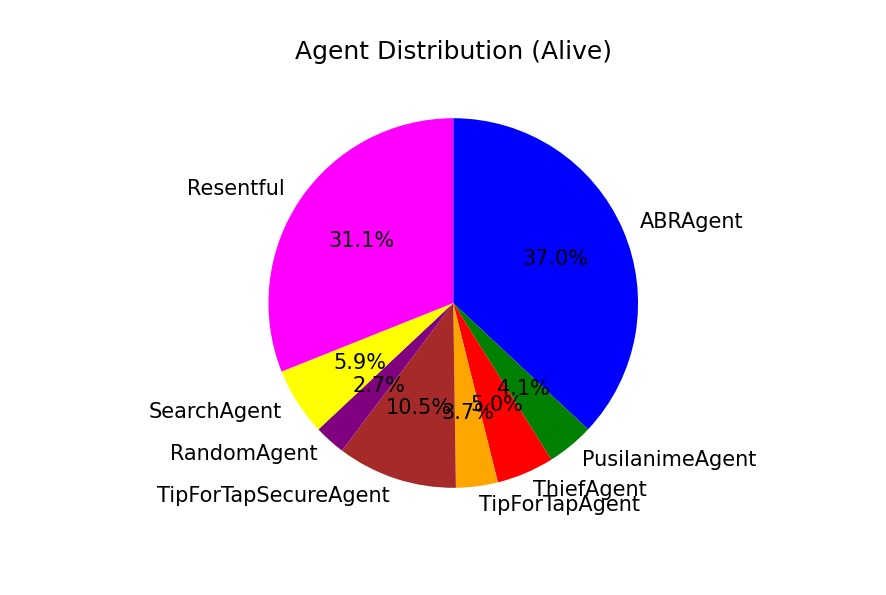
\includegraphics[width=\textwidth]{population_1.jpg}
      \end{minipage}\hfill
      \begin{minipage}{0.32\textwidth}
            \centering
            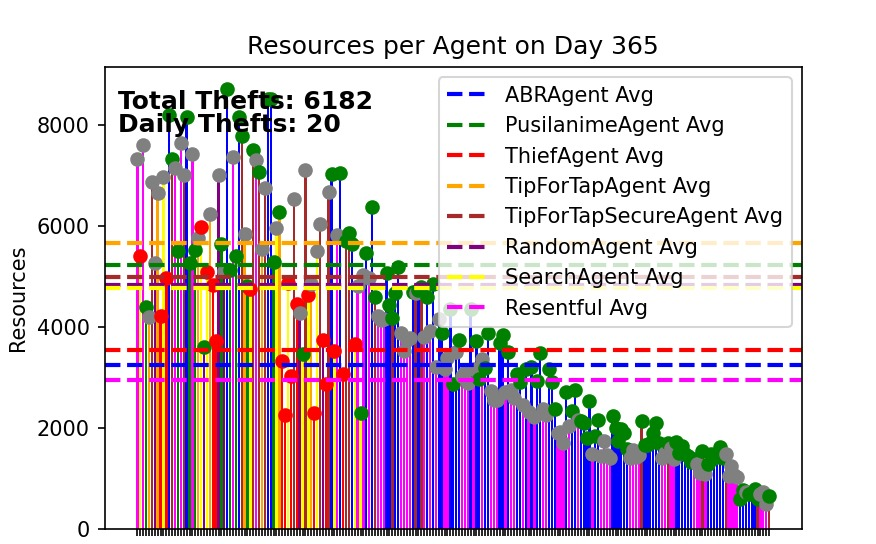
\includegraphics[width=\textwidth]{agents_1.jpg}
      \end{minipage}\hfill
      \begin{minipage}{0.32\textwidth}
            \centering
            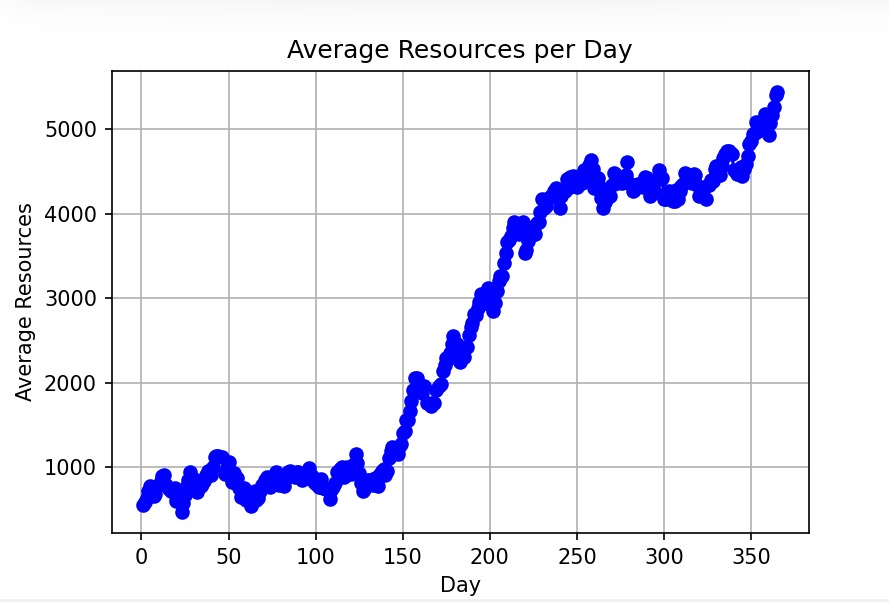
\includegraphics[width=\textwidth]{resources_1.jpg}
      \end{minipage}
\end{figure}


\subsection{Menor tolerancia al robo}
\subsubsection{Configuraci\'on inicial}
\begin{itemize}
      \item Cantidad de agentes iniciales: 50 (distribuidos aleatoriamente)
      \item P\'erdida de recursos por d\'{\i}a: 100
      \item Cantidad de recursos iniciales: Un n\'umero random entre 300 y 600.
      \item Tolerancia al robo: 0.5 - 0.
      \item Frecuencia de reproducci\'on: 20 d\'{\i}as.
      \item Densidad de reproducci\'on: 10
      \item Ruido: 0.1
\end{itemize}
\subsubsection{Resultados}
Con una menor toleracia al robo los Always cooperate no demoraron en desaparecer y a medida que se acerca a 0 los profetas también la pasan mal pudiendo llegara desaparecer
en algunas ocasiones. A medida que la tolerancia al robo disminuye el judge domina en porcentaje poblacional con casi la mitad, aunque sigue siendo de los que mas bajos recursos
tienen en promedio, el tit for tat sigue ganando a nivel de recursos, pero a medida que la tolerancia se acerca a 0, casi nadie tiene permitido robar y los pobladores que dominan
son los que tienden a cooperar mas como el tit for tat o el always cooperate a nivel poblacional, pero por supuesto a nivel de recursos no distan muchos de otros. Aunque ahora que todos
se ven obligados a cooperar por la autoridad ganan en promedio una mayor cantidad de recursos, sobre los 8500 en promedio.
\subsubsection{Gr\'aficas}
\begin{figure}[h]
      \centering
      \begin{minipage}{0.42\textwidth}
            \centering
            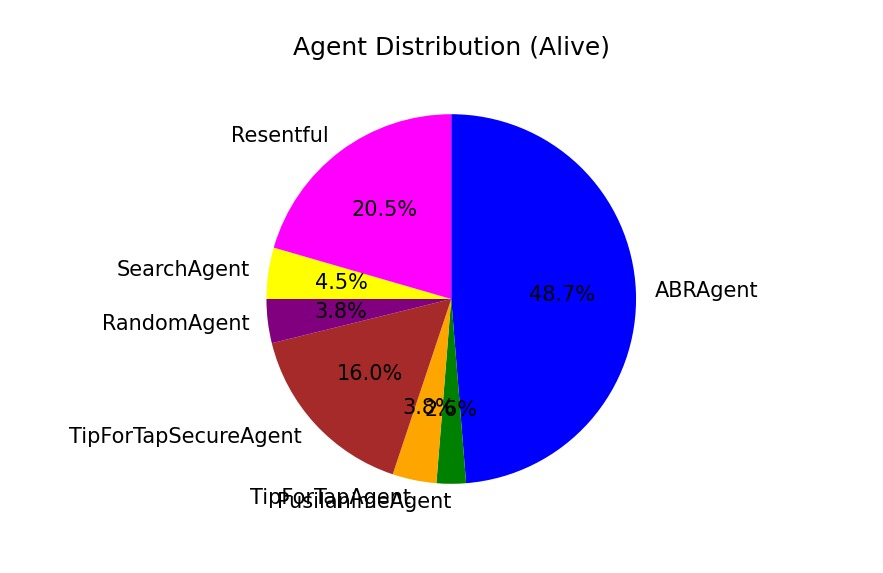
\includegraphics[width=\textwidth]{population_2.jpg}
            \caption{Tolerancia al robo = 0.5}
      \end{minipage}\hfill
      \begin{minipage}{0.42\textwidth}
            \centering
            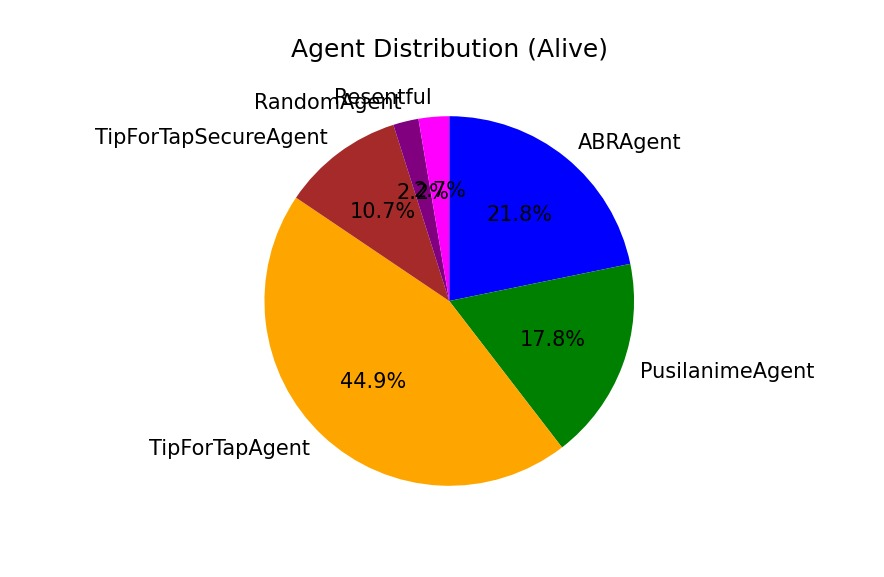
\includegraphics[width=\textwidth]{population_3.jpg}
            \caption{Tolerancia al robo cercana a 0}
      \end{minipage}\hfill
\end{figure}


\subsection{Mayor Ruido}
\subsubsection{Configuraci\'on inicial}
\begin{itemize}
      \item Cantidad de agentes iniciales: 50 (distribuidos aleatoriamente)
      \item P\'erdida de recursos por d\'{\i}a: 100
      \item Cantidad de recursos iniciales: Un n\'umero random entre 300 y 600.
      \item Tolerancia al robo: 1.
      \item Frecuencia de reproducci\'on: 20 d\'{\i}as.
      \item Densidad de reproducci\'on: 10
      \item Ruido: 0.3 - 0.5
\end{itemize}

\subsubsection{Resultados}
A medida que aumenta la falta de comunicaci\'on y entendimiento en la sociedad, se hace m\'as dif\'{\i}cil no solo predecir para los agentes que posible acci\'on van a tomar
los dem\'as, sino que se les dificulta que los dem\'as entiendan sus acciones. Por lo tanto el avance de la sociedad es m\'as lenta, les cuesta el doble de tiempo reunir la misma
cantidad de recursos que con el ruido = 0.1. Y a medida que el ruido se acerca a 0.5 se hace cada vez m\'as probable que la sociedad se destruya a s\'{\i} misma y mueran todos los
pobladores, en general pueden durar hasta solo 60 d\'ias en el peor de los casos. Lo c\'ual evidencia que en esta simulación y en la vida real, entenderse es importante.

\subsection{Modificando la poblaci\'on}
\subsubsection{Configuraci\'on inicial}
\begin{itemize}
      \item Cantidad de agentes iniciales: 50 (quitando al judge y al resentido)
      \item P\'erdida de recursos por d\'{\i}a: 100
      \item Cantidad de recursos iniciales: Un n\'umero random entre 300 y 600.
      \item Tolerancia al robo: 1.
      \item Frecuencia de reproducci\'on: 20 d\'{\i}as.
      \item Densidad de reproducci\'on: 10
      \item Ruido: 0.1
\end{itemize}

\subsubsection{Resultados}
En esta configuraci\'on al haber m\'as aldeanos que tienen como opci\'on robar se empiezan a traicionar unos a otros y explotando a los que cooperan. Desencadenando una disminuci\'on de la
poblaci\'on en los primeros 50 d\'{\i}as, despu\'es cuando se matan unos a otros, los pocos sobrevivientes cooperan entre si y gracias la descendencia las estrategias buenas repoblan la aldea.
Por supuesto, la ganancia de la aldea en cuesti\'on de recursos es muy pobre llegando apenas a los 2500.

\subsubsection{Gr\'aficas}
\begin{figure}[h]
      \centering
      \begin{minipage}{0.42\textwidth}
            \centering
            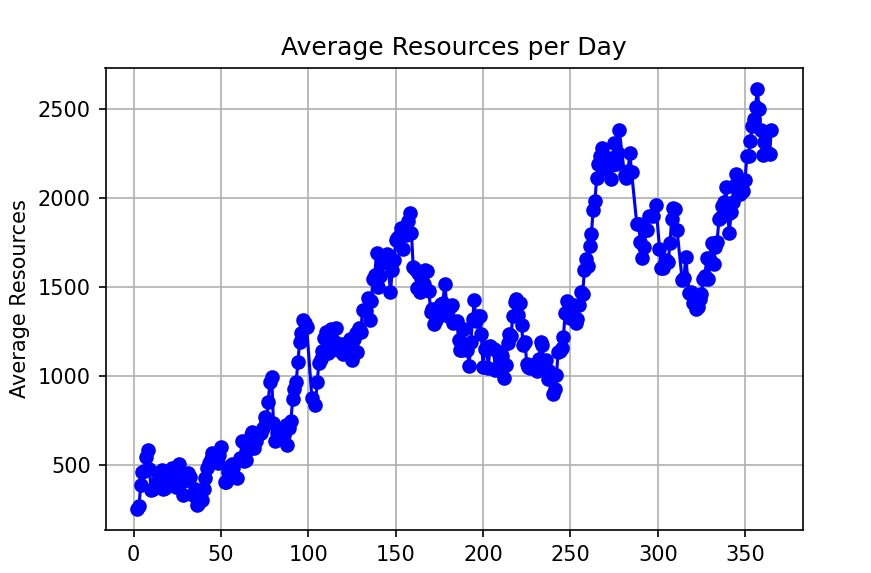
\includegraphics[width=\textwidth]{resources_2.jpg}
      \end{minipage}\hfill
      \begin{minipage}{0.42\textwidth}
            \centering
            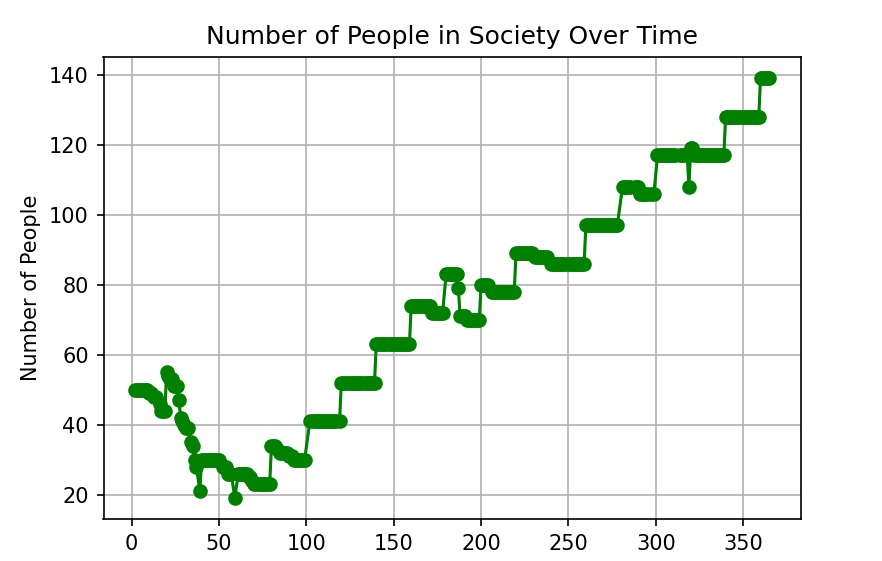
\includegraphics[width=\textwidth]{alive_1.jpg}
      \end{minipage}\hfill
\end{figure}


\subsection{Modificando la poblaci\'on 2.0}
\subsubsection{Configuraci\'on inicial}
\begin{itemize}
      \item Cantidad de agentes iniciales: 50 (entre always cheat y judge)
      \item P\'erdida de recursos por d\'{\i}a: 100
      \item Cantidad de recursos iniciales: Un n\'umero random entre 300 y 600.
      \item Tolerancia al robo: 1.
      \item Frecuencia de reproducci\'on: 20 d\'{\i}as.
      \item Densidad de reproducci\'on: 10
      \item Ruido: 0.1
\end{itemize}

\subsubsection{Resultados}
Despu\'es de varios d\'{\i}as los always cheat perdieron la cofianza de los judges y ahora los judges trabajan por su cuenta, mientras que los ladrones solo les queda la opci\'on de matarse
entre ellos, disminuyendo mucho su poblaci\'on. Cuando ya quedan pocos ladrones los judges se dan cuenta que aunque caigan en un grupo con los ladrones les da m\'as ganancia cooperar que ir
por su cuenta, y asi los always cheat pueden respirar y vivir un poco. Esta simulación termina con una coexistencia en la que los judges toleran a los ladrones por que son pocos y les es m\'as
beneficioso colaborar aunque hayan algunos que roben, y los ladrones se sustentan en bajos n\'umeros robando. Aunque se nota que la media de recursos alcanzada por ambas partes es muy diferente.

\subsubsection{Gr\'aficas}
\begin{figure}[h]
      \centering
      \begin{minipage}{0.42\textwidth}
            \centering
            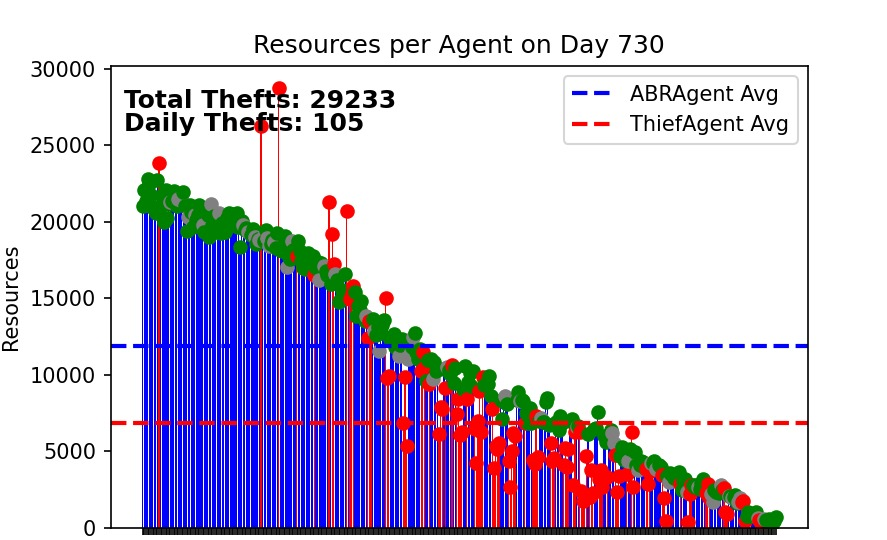
\includegraphics[width=\textwidth]{agents_2.jpg}
      \end{minipage}\hfill
      \begin{minipage}{0.42\textwidth}
            \centering
            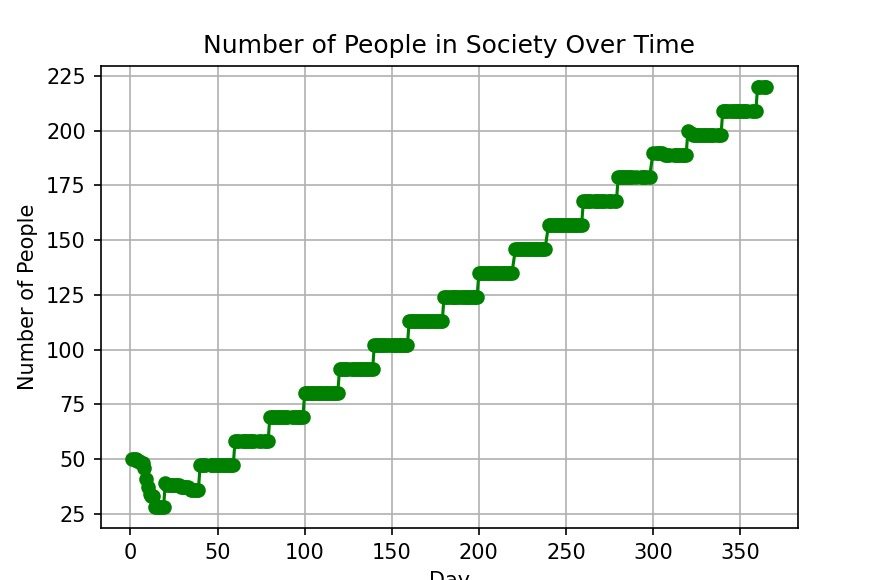
\includegraphics[width=\textwidth]{alive_2.jpg}
      \end{minipage}\hfill
\end{figure}

\newpage

\section{El Edena Ruh}
El edena ruh es un artista itinerante que pasa por el pueblo todos los años, se entera de lo que ha pasado en el pueblo y luego va a contar esas historias por el mundo.
Sin otro medio de comunicaci\'on en la aldea, la \'unica forma en la que viaja la informaci\'on es a trav\'es de las historias. Y a veces las historias viajan m\'as rapido
que las personas. Por supuesto, si el Edena adorna un poco las historias de la aldea para llamar la atenci\'on de los oyentes a nadie le molestar\'{\i}a ni un poco.

\subsection{El prompt}
Entrando ahora un poco en detalles t\'ecnicos y de implementaci\'on, el Edena Ruh no es m\'as que el LLM de Google, Gemini Advanced. La simulación genera unos logs con toda la
informaci\'on de cada ronda. Al terminar la simulación esos logs se le mandana Gemini con la siguiente estructura de prompt:
\begin{itemize}
      \item Se le explica que tenemos como objetivo simular una sociedad y se le explican los detalles de la simulación, como funciona y las reglas que tiene.
      \item Se le da una lista con los nombres y las estrategias de los jugadores.
      \item Se le dan los logs de la simulación y se le dice que debe inventar una historia teniendo en cuenta el contexto anterior, la historia debe tener política, romance,
            aventura y personajes relevantes.
      \item Se le pide que sea fiel a la informaci\'on que esta en el log, que sea creativa y que escriba la historia en espa\~nol.
\end{itemize}

\subsection{La historia}
\vspace*{5mm}
\begin{tcolorbox}[enhanced, breakable,skin first=enhanced, skin middle=enhanced, skin last=enhanced]
      El Nacimiento de Neotopia: Una Saga de Supervivencia y Estrategia
      \textbf{Día 1: El Comienzo Incierto}\\
      En el año 2142, tras el colapso de la civilización, un grupo de 100 supervivientes se une para formar Neotopia, un refugio en medio de la desolación. La vida es un
      juego de azar, donde los recursos son escasos y la confianza, un lujo. Cada día trae consigo un evento, una oportunidad para prosperar o caer en la miseria. La
      supervivencia depende de las decisiones que tomen, ya sea cooperar, explotar o mantenerse al margen en los eventos cooperativos. Entre los habitantes se destacan
      Anya (Agente Pusilánime \#1), una joven idealista que cree en la bondad innata de las personas, y Kael (Agente ABR \#24), un estratega pragmático que analiza cada
      situación con frialdad. El destino los une en el primer evento cooperativo, donde sus elecciones divergen: Anya coopera, mientras Kael se mantiene al margen.
      \\\textbf{Día 5: El Amor en Tiempos Difíciles}\\
      La vida en Neotopia es dura, pero el amor encuentra su camino. Anya y Kael, a pesar de sus diferencias, se sienten atraídos el uno por el otro. Su relación florece
      en medio de la incertidumbre, un rayo de luz en la oscuridad.
      \\\textbf{Día 20: La Traición de Kael}\\
      La desconfianza corroe a Kael. Durante un evento cooperativo, sucumbe a la tentación y explota a su grupo. Anya, devastada por la traición de su amado, se aleja de
      él. La comunidad se divide entre aquellos que apoyan a Anya y los que justifican las acciones de Kael.
      \\\textbf{Día 30: La Gran Prueba}\\
      Una tormenta de fuego azota Neotopia, poniendo a prueba la resiliencia de sus habitantes. Los recursos se vuelven negativos, lo que significa que todos perderán algo,
      pero la cooperación es crucial para minimizar las pérdidas. Kael, atormentado por la culpa, se redime liderando los esfuerzos de reconstrucción. Su valentía y sacrificio
      le ganan el respeto de la comunidad, incluso el de Anya.
      \\\textbf{Día 50: Un Nuevo Comienzo}\\
      Neotopia se levanta de las cenizas, más fuerte y unida. Anya y Kael, reconciliados, se convierten en líderes respetados. La comunidad aprende a equilibrar la cooperación
      y la estrategia, representada por la creciente popularidad del Agente Search, que simula futuros movimientos para tomar la mejor decisión.
      \\\textbf{El Auge de la Política}\\
      La necesidad de organización lleva a la formación de facciones políticas. Anya lidera a los idealistas, abogando por la cooperación y la compasión. Kael encabeza a los
      pragmáticos, promoviendo la estrategia y el análisis. La tensión entre ambos bandos aumenta, creando un drama político apasionante.
      \\\textbf{Día 100: La Tragedia Golpea}\\
      Un evento especial trae consigo una pérdida masiva de recursos. La comunidad se tambalea al borde del colapso. Algunos, como el Agente Ladrón \#92, aprovechan el caos
      para robar, mientras que otros, como Anya, se mantienen firmes en su compromiso con la cooperación.
      \\\textbf{El Resurgimiento de Neotopia}\\
      La comunidad se recupera de la tragedia, pero las cicatrices permanecen. La desconfianza hacia los agentes aleatorios y ladrones crece, y algunos, como el Agente \#30, son excluidos de los eventos cooperativos. La historia de Neotopia es una montaña rusa de emociones, donde la política, el romance y la aventura se entrelazan en una lucha épica por la supervivencia. Los personajes principales, Anya y Kael, representan dos enfoques diferentes pero igualmente válidos para enfrentar la adversidad. Su relación, puesta a prueba por la traición y la redención, es un recordatorio de que incluso en los momentos más oscuros, el amor y la esperanza pueden prevalecer.

      \textbf{Personajes Icónicos:}
      \begin{itemize}
            \item Anya (Agente Pusilánime \#1): La voz de la compasión y la esperanza, líder de los idealistas.
            \item Kael (Agente ABR \#24): El estratega frío y calculador, líder de los pragmáticos.
            \item Agente Ladrón \#92: El oportunista que se aprovecha del caos, generando desconfianza y conflicto.
            \item Agente Search: El visionario que utiliza la tecnología para predecir el futuro y tomar decisiones estratégicas.
            \item Agente \#30: El marginado, excluido de los eventos cooperativos debido a su baja reputación, un recordatorio de las duras consecuencias de la traición.
      \end{itemize}
      La simulación, con sus altibajos, refleja la complejidad de la sociedad humana. A través de los eventos especiales y cooperativos, vemos cómo las decisiones individuales pueden tener un impacto profundo en el destino de la comunidad. La historia de Neotopia nos recuerda que la supervivencia no se trata solo de fuerza o inteligencia, sino también de compasión, estrategia y la capacidad de adaptarse a un mundo en constante cambio.

\end{tcolorbox}
\newpage
\section{Conclusiones}
Este proyecto tenia tres objetivos a los que aspir\'abamos. El primero era enfocar nuestros conocimientos de simulación para poder simular una variante del juego del prisionario
tratando de simular una civilización, o al menos que se pueda ver una correlaci\'on entre las dos cosas. Modelando el entorno y los agentes como lo hicimos creo que nos acercamos
al menos un poco al objetivo, a\~nadiendo mec\'anicas adicionales con tal de acercarnos lo m\'as posible  a una civilización. Por supuesto estamos muy lejos de lograr realmente eso,
simular una civilización es algo mucho mas complejo y completo que esto, pero creo que el acercamiento no fue malo a partir de la idea del dilema del prisionero. El segundo objetivo
era usar nuestros conocimientos de IA para idear estrategias que sean capaces de participar competitivamente en el juego. Con este fin logramos crear varios agentes inteligentes con
resultados favorables en el juego, no lograron ganarle al tit for tat en muchos escenarios, pero mostraron una actuaci\'on competente en muchos otros, sobre todo el judge. Nuestro tercer
y \'ultimo objetivo era encontrar una similitud entre este juego, con sus estrategias y mec\'anicas con el real comportamiento de las personas en sociedad, tratando de relacionar la mejor
estrategia del juego con la mejor estrategia de comportarse en la vida real, para cada uno y para la sociedad. Intentamos que las mec\'anicas de la simulaci\'on se correspondieran con hechos
o situaciones de la vida real en sociedad, como son la falta de comunicaci\'on, la tolerancia al robo, la idea de que hay m\'as opciones que solo cooperar o robar, el hecho de una reputaci\'on y
la confianza entre individuos.

Gracias a los resultados de la simulaci\'on hemos podido ver la importancia que tiene el ruido en la obstaculizaci\'on del avance de la sociedad, ilustrando la importancia de la comunicaci\'on
efectiva. El papel de las instituciones y reglas representado con la tolerancia al robo, como impacta en la conducta social y la toma de decisisones de las personas, y en general como la toma de una soluci\'on
m\'as egoista no siempre es la que trae mayor beneficioso para el individio. Podr\'iamos decir que el dilema del prisionero nos muestra que la forma m\'as efectiva de ser egoista es cooperar.

\end{document}